\documentclass[12pt, dutch]{article}
\usepackage{hyperref}
\usepackage{graphicx}
\usepackage{subcaption}
\hypersetup{
    colorlinks=true,
    linkcolor=black,
    filecolor=magenta,      
    urlcolor=blue,
    pdfpagemode=FullScreen,
    }
\urlstyle{same}
\title{HASH1: Hashtabel search-hits en misses}
\author{Manoah Kinnaert}
\begin{document}

\begin{titlepage}
    \maketitle
\end{titlepage}
\pagebreak
\section{Korte inleiding}

\section{Bevindingen}
\begin{figure}[htbp]
    \centering
    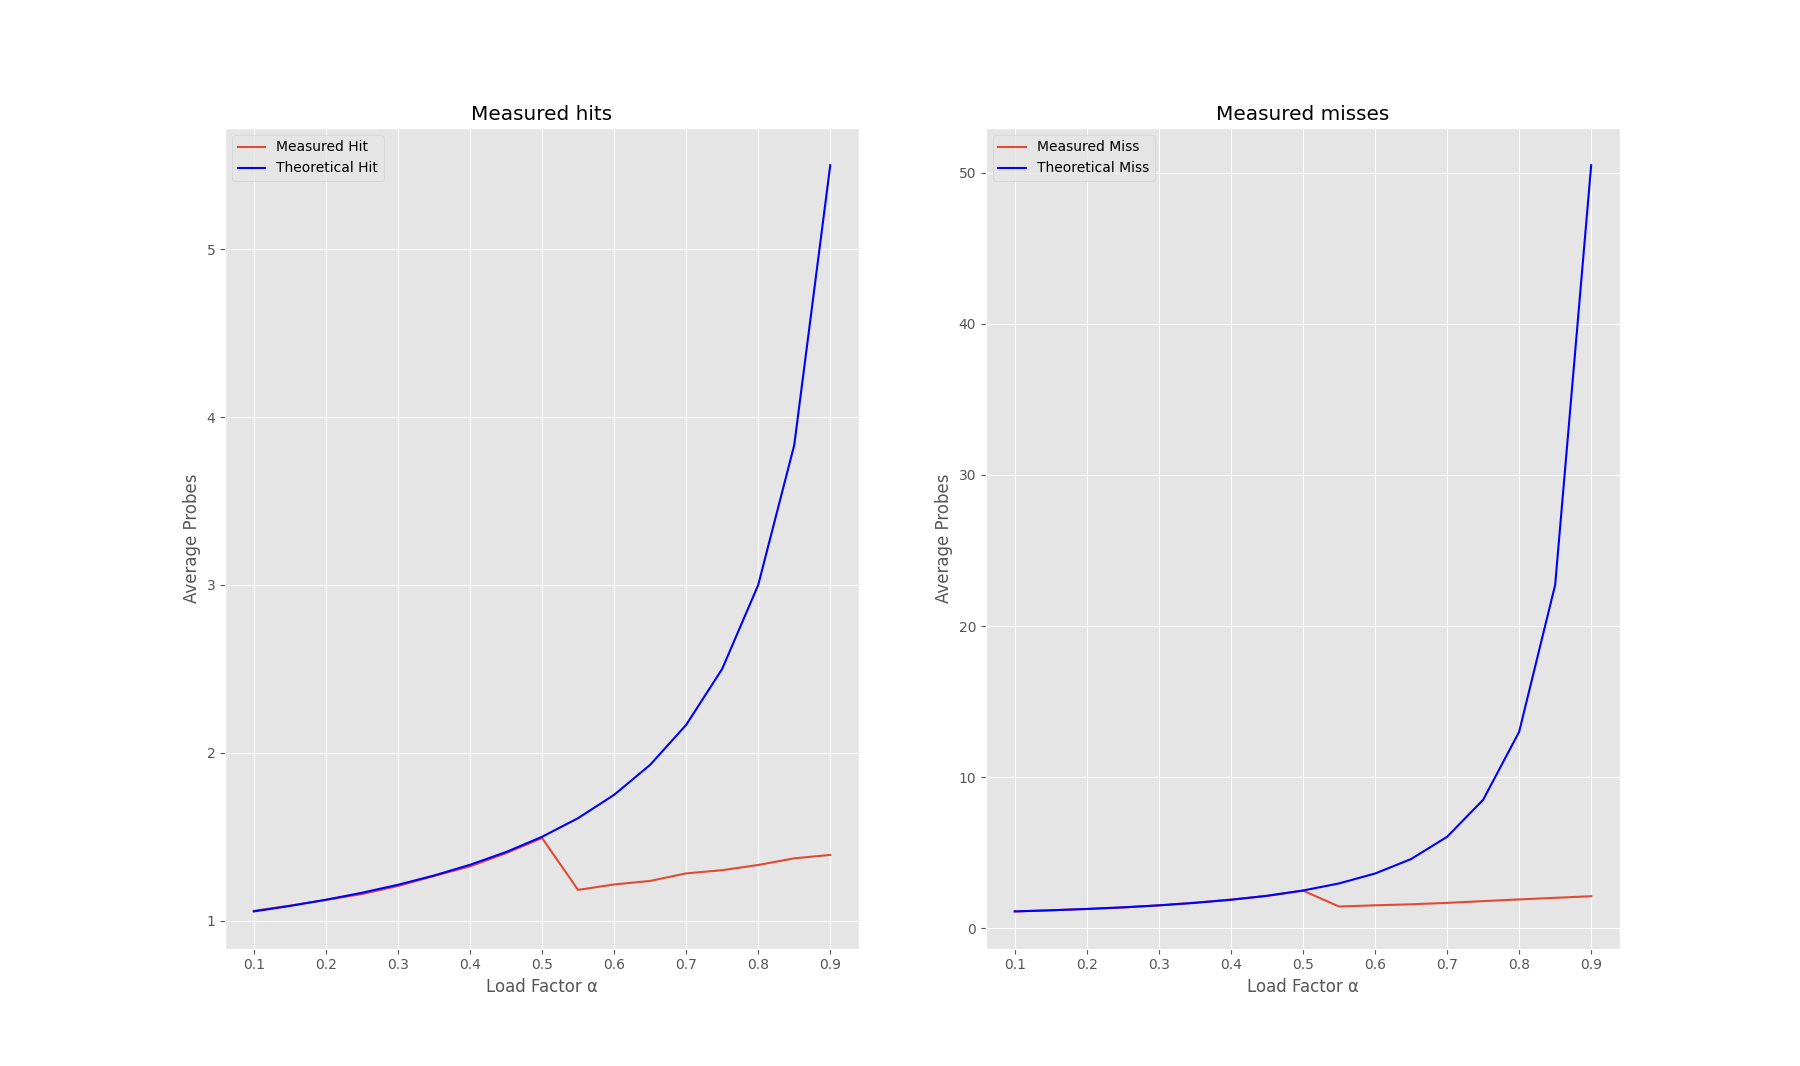
\includegraphics[width=0.9\textwidth]{../../images/hash1/chart.png}
    \caption{Hashtabel searh-hits en search-misses (indien niet duidelijk genoeg zie git repo)}
    \label{fig:heap_insert_1}
\end{figure}

\end{document}